%! TeX program = lualatex
\documentclass[../main.tex]{subfiles}
\begin{document} \section{Scaling, isometry and allometry}
In Example~\ref{ex:toucan}, we made an assumption about the scaling relation between lengths of birds and their volume. This assumption results in an \hlwarn{outlier} which simply does not fit our model.

\begin{minipage}{.5\textwidth}
  \includegraphics{../standalones/build/plot-birds-of-costa-rica}
\end{minipage}
\begin{minipage}{.5\textwidth}
  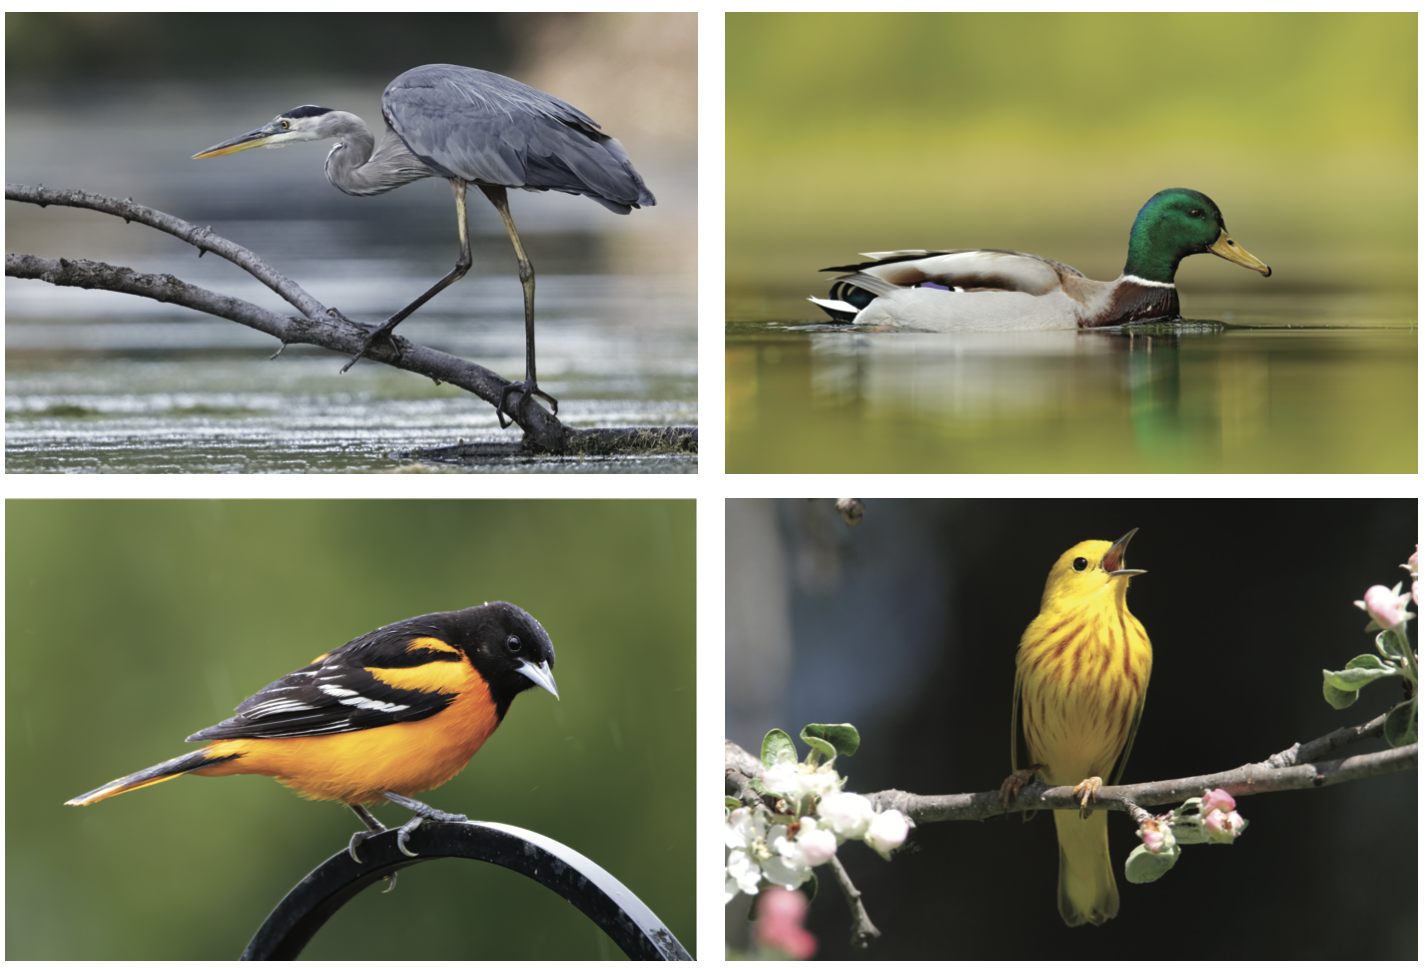
\includegraphics[width=\textwidth]{../standalones/image-birds.png}

  {\footnotesize{} Images reproduced under the terms of the Enhanced Licensing agreement, Adobe Inc.}
\end{minipage}

Can you guess which of the above birds correspond to the outlying data point? 
\blanklines{3}

What is this assumption?
% these birds have similar density with respect to a cube.
\blanklines{10}

If we use our model to predict the weight of the outlier, should we expect an accurate answer?
\blanklines{5}

What caveats should accompany our model and its predictions?
% we cannot apply our model to predict weight of birds of ALL shapes and sizes. We need to limit our model 
\blanklines{5}

\clearpage
Let's build some vocabulary for building simple models using scaling relations, c.f. Example~\ref{ex:toucan}.

\begin{mdframed}[style=simple-compact]
  If two quantities \(x,y\) are related by a \hlattn{linear} relation \(y = c x\) for some constant \(c > 0\), then we say \hlmain{\(x\) and \(y\) exhibit isometry}.

  If two quantities \(x,y\) are related by a \hlattn{non-linear} relation, i.e., \(y = c x^{\alpha}\) for some constant \(c > 0\) and \(\alpha \ne 1\), then we say \hlmain{\(x\) and \(y\) exhibit allometry}.
\end{mdframed}

\begin{example}
  Consider lengths, volumes and weights of birds as discussed in Example~\ref{ex:toucan}.

  \begin{enumerate}[wide]
    \item Do length and weight exhibit isometry or allometry? Explain your reasoning.
      \blanklines{10}

    \item Do volume and weight exhibit isometry or allometry? Explain your reasoning.
      \blanklines{10}
  \end{enumerate}
\end{example}

The purpose of the next example is to understand the phrase ``\emph{by what factor does \ldots{}}.''
\begin{example}
  If we double the diameter of a circle, then by what factor do we expect its area to increase? Support your reasoning with calculations.
  \blanklines{12}
\end{example}

\clearpage
Let's tie everything together and wrap up the introduction week with a comprehensive modelling exercise using scaling relations.
\begin{example}
  A team of palaeontologists has discovered two \emph{Tyrannosaurus rex} footprints. The first measures \(85\) cm in length and the second measures \(70\) cm in length, suggesting they were made by different dinosaurs. 

  \begin{enumerate}[wide]
    \item Based on these footprints, predict how much heavier the first dinosaur was.

      \blanklines{25}

    \item What assumptions did you make? What caveats should accompany your prediction?
      \blanklines{10}

    \item Given footprint data of a T. rex and a Diplodocus, should you be confident comparing their weights in the same way? Articulate your reasoning.
      \blanklines{5}
  \end{enumerate}
\end{example}
\end{document}
